\documentclass[12pt]{amsart}
% packages
\usepackage{graphicx}
\usepackage{setspace}
\usepackage{amssymb,amsmath,amsthm,amsfonts,amscd}
\usepackage{hyperref}
\usepackage{color}
\usepackage{booktabs}
\usepackage{tabularx}
\usepackage{enumitem}
\usepackage[retainorgcmds]{IEEEtrantools}
\usepackage[notref,notcite,final]{showkeys}
\usepackage[final]{pdfpages}
\usepackage{fancyhdr}
\usepackage{upgreek}
\usepackage{multicol}

\usepackage{fancyvrb}
\usepackage{listings}
% set margin as 0.75in
\usepackage[margin=0.75in]{geometry}

% tikz-related settings
\usepackage{tikz}
\usepackage{tikz-cd}
\usetikzlibrary{cd}

% theorem environments with italic font
\newtheorem{thm}{Theorem}[section]
\newtheorem*{thm*}{Theorem}
\newtheorem{lemma}[thm]{Lemma}
\newtheorem{prop}[thm]{Proposition}
\newtheorem{claim}[thm]{Claim}
\newtheorem{corollary}[thm]{Corollary}
\newtheorem{conjecture}[thm]{Conjecture}
\newtheorem{question}[thm]{Question}
\newtheorem{procedure}[thm]{Procedure}
\newtheorem{assumption}[thm]{Assumption}

% theorem environments with roman font (use lower-case version in body
% of text, e.g., \begin{example} rather than \begin{Example})
\newtheorem{Definition}[thm]{Definition}
\newenvironment{definition}
{\begin{Definition}\rm}{\end{Definition}}
\newtheorem{Example}[thm]{Example}
\newenvironment{example}
{\begin{Example}\rm}{\end{Example}}

\theoremstyle{definition}
\newtheorem{remark}[thm]{\textbf{Remark}}

% special sets
\newcommand{\A}{\mathbb{A}}
\newcommand{\C}{\mathbb{C}}
\newcommand{\F}{\mathbb{F}}
\newcommand{\N}{\mathbb{N}}
\newcommand{\Q}{\mathbb{Q}}
\newcommand{\R}{\mathbb{R}}
\newcommand{\Z}{\mathbb{Z}}
\newcommand{\cals}{\mathcal{S}}
\newcommand{\ZZ}{\mathbb{Z}_{\ge 0}}
\newcommand{\cala}{\mathcal{A}}
\newcommand{\calb}{\mathcal{B}}
\newcommand{\cald}{\mathcal{D}}
\newcommand{\calh}{\mathcal{H}}
\newcommand{\call}{\mathcal{L}}
\newcommand{\calr}{\mathcal{R}}
\newcommand{\la}{\mathbf{a}}
\newcommand{\lgl}{\mathfrak{gl}}
\newcommand{\lsl}{\mathfrak{sl}}
\newcommand{\lieg}{\mathfrak{g}}

% math operators
\DeclareMathOperator{\kernel}{\mathrm{ker}}
\DeclareMathOperator{\image}{\mathrm{im}}
\DeclareMathOperator{\rad}{\mathrm{rad}}
\DeclareMathOperator{\id}{\mathrm{id}}
\DeclareMathOperator{\hum}{[\mathrm{Hum}]}
\DeclareMathOperator{\eh}{[\mathrm{EH}]}
\DeclareMathOperator{\lcm}{\mathrm{lcm}}
\DeclareMathOperator{\Aut}{\mathrm{Aut}}
\DeclareMathOperator{\Inn}{\mathrm{Inn}}
\DeclareMathOperator{\Out}{\mathrm{Out}}
\DeclareMathOperator{\Gal}{\mathrm{Gal}}


% frequently used shorthands
\newcommand{\ra}{\rightarrow}
\newcommand{\se}{\subseteq}
\newcommand{\ip}[1]{\langle#1\rangle}
\newcommand{\dual}{^*}
\newcommand{\inverse}{^{-1}}
\newcommand{\norm}[2]{\|#1\|_{#2}}
\newcommand{\abs}[1]{\lvert #1 \rvert}
\newcommand{\Abs}[1]{\bigg| #1 \bigg|}
\newcommand\bm[1]{\begin{bmatrix}#1\end{bmatrix}}
\newcommand{\op}{\text{op}}

% nicer looking empty set
\let\oldemptyset\emptyset
\let\emptyset\varnothing

\setlist[enumerate,1]{topsep=1em,leftmargin=1.8em, itemsep=0.5em, label=\textup{(}\arabic*\textup{)}}
\setlist[enumerate,2]{topsep=0.5em,leftmargin=3em, itemsep=0.3em}

%pagestyle
%\pagestyle{fancy} 

\begin{document}
\begin{center}
    \textsc{Random Walks. HW 1\\ Ian Jorquera\\ Collaboration: Tristan Neighbors}
\end{center}
\vspace{1em}


\definecolor{codegreen}{rgb}{0,0.6,0}
\definecolor{codegray}{rgb}{0.5,0.5,0.5}
\definecolor{codepurple}{rgb}{0.58,0,0.82}
\definecolor{backcolour}{rgb}{1,1,1}

\lstdefinestyle{mystyle}{
    backgroundcolor=\color{backcolour},   
    commentstyle=\color{codegray},
    keywordstyle=\color{magenta},
    numberstyle=\tiny\color{codegray},
    stringstyle=\color{codegreen},
    basicstyle=\ttfamily\footnotesize,
    breakatwhitespace=false,         
    breaklines=true,                 
    captionpos=b,                    
    keepspaces=true,                 
    numbers=left,                    
    numbersep=5pt,                  
    showspaces=false,                
    showstringspaces=false,
    showtabs=false,                  
    tabsize=2
}

\lstset{style=mystyle}


\begin{itemize}
\item[(1)] The probability density function for the Cauchy distribution is $p(x)=\frac{b}{\pi}\frac{1}{b^2+x^2}$. whose characteristic equation is 
$$\lambda(k)=\int_{-\infty}^{\infty}e^{ikx}\frac{b}{\pi}\frac{1}{b^2+x^2}dx=e^{-b|k|}$$ This was computed with Wolfram Alpha Fourier Transform Calculator(which adds an additional normalizing factor that I ignored).\\
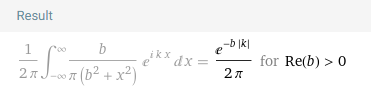
\includegraphics[scale=.5]{rw-p1-int.png}

Now to get the characteristic function after $n$ steps we can multipy the characteristic function after $1$ step to find that $\lambda^n(k)=\left(e^{-b|k|}\right)^n=e^{-nb|k|}$. Notice that this is the characteristic function of the Cauchy distribution with $b\ra nb$. That is $P_n(x)=\frac{nb}{\pi}\frac{1}{(nb)^2+x^2}$.\\

\item[(2)] In this case let $\textbf{r}=r_x{\hat{\textbf{x}}}+r_y{\hat{\textbf{y}}}=(r_x,r_y)$. We have the probability distribution:
$$p(r)=\begin{cases}
    \frac{1}{4} & \textbf{r}=1{\hat{\textbf{x}}}\\
    \frac{1}{4} & \textbf{r}=1{\hat{\textbf{y}}}\\
    \frac{1}{4} & \textbf{r}=-1{\hat{\textbf{x}}}\\
    \frac{1}{4} & \textbf{r}=-1{\hat{\textbf{y}}}\\
\end{cases}$$
Where we can compute the characteristic function as 
$\lambda(\Theta)=\ip{e^{i\Theta \textbf{r}}}=\frac{1}{4}e^{i\theta_x}+\frac{1}{4}e^{i\theta_y}+\frac{1}{4}e^{-i\theta_x}+\frac{1}{4}e^{-i\theta_y}$. Notice that $e^{i\theta_x}+e^{-i\theta_x}=2\cos(\theta_x)$ and similarly $e^{i\theta_y}+e^{-i\theta_y}=2\cos(\theta_y)$. So $\lambda(\Theta)=\frac{1}{2}(\cos(\theta_x)+\cos(\theta_y))$.\\

\item[(3)] let $p(\textbf{r})=\frac{1}{2\pi l}\delta(r-l)$
let $\textbf{k}=(k,\phi)$ and $\textbf{r}=(r,\theta)$ be in polar coordinates, in which case we can determine that the characteristic function is 
$$\lambda(\textbf{k})=\int_{-\infty}^{\infty}\int_{-\infty}^{\infty}p(\textbf{r})e^{i\textbf{k}\textbf{r}}d^2\textbf{r}$$
In polar coordinates this is 
$$\lambda(\textbf{k})=\int_{-\pi}^{\pi}\int_{0}^{\infty}\frac{1}{2\pi l}\delta(r-l)e^{ikr\cos(\theta-\phi)}r\,dr\,d\theta=\int_{0}^{2\pi}\frac{1}{2\pi l}\int_{0}^{\infty}\delta(r-l)e^{ikr\cos(\theta-\phi)}r\,dr\,d\theta$$
Notice that we can re shift the integral over $\theta$ which allows us to treat $\theta-\phi\ra\theta$ so we can rewrite $\theta-\phi$ with not change to the integral(Formally this is a u-substitution). For the inner integral recall that $\int_{-\infty}^{\infty}f(x)\delta(x-l)dx=f(l)$ so we can plug in for $r=l$ and cancel terms so we know that 
$$\lambda(\textbf{k})=\frac{1}{2\pi }\int_{0}^{2\pi}e^{ikl\cos(\theta)}\,d\theta=J_0(kl)$$
From the internet(this source \href{https://encyclopediaofmath.org/wiki/Bessel_functions}{here}) we can write the Bessel function as a Taylor series $J_0(kl)=1-\left(\frac{kl}{2}\right)^2+o(k^4)$.
Because we are only concerned with asymptotic behavior we will assume $k$ is small, so we may consider the quadratic Taylor approximation $\lambda(\textbf{k})=1-\left(\frac{kl}{2}\right)^2=\exp(-\frac{1}{4}k^2l^2)=\exp(-\frac{1}{4}\textbf{k}^\intercal \Sigma \textbf{k})$ where $\Sigma=\begin{pmatrix} l^2/2 & 0\\ 0 & l^2/2 \end{pmatrix}$, where $\textbf{k}$ is now in Cartesian coordinates.\\

According to Wikipedia(Source: \href{https://en.wikipedia.org/wiki/Multivariate_normal_distribution}{here}) this is the characteristic function of the mean zero multivariate normal density function $\mathcal{N}(0, \Sigma)$.\\

Now notice that $\lambda(\textbf{k})^n=\exp(-\frac{1}{2}\textbf{k}^\intercal \Sigma \textbf{k})^n=\exp(-\frac{1}{2}\textbf{k}^\intercal n\Sigma \textbf{k})$ where $n\Sigma=\begin{pmatrix} nl^2/2 & 0\\ 0 & nl^2/2 \end{pmatrix}$, which means that $P_n(\textbf{x})=\det(2\pi n\Sigma)^{-\frac{1}{2}}\exp(-\frac{1}{2}\textbf{x}^\intercal n\Sigma \textbf{x})=\frac{1}{\sqrt{\pi}nl^2}\exp(-\frac{1}{2}\textbf{x}^\intercal n\Sigma \textbf{x})$.\\


\item[(4)] Let $p(\textbf{r})=\frac{1}{2\pi r}e^{-r}$. We can compute the characteristic function using polar coordinates as
$$\lambda(\textbf{k})=\int_{0}^{2\pi}\int_{0}^{\infty} \frac{1}{2\pi r}e^{-r}e^{ikr\cos(\theta)}r\,dr\,d\theta=\frac{1}{2\pi }\int_{0}^{2\pi}\int_{0}^{\infty} e^{-r}e^{ikr\cos(\theta)}\,dr\,d\theta$$
Again we are rotating $\theta-\phi$ to $\theta$ and which does not affect the integral as it is radially symmetric. We can compute The inner integral using wolfram alpha to find that
$$\int_{0}^{2\pi}\int_{0}^{\infty} \frac{1}{2\pi r}e^{-r}e^{ikr\cos(\theta)}r\,dr\,d\theta=\frac{1}{2\pi}\int_{0}^{2\pi} \frac{1}{1-ik\cos(\theta)}\,d\theta$$
$$=\frac{1}{2\pi}\int_{0}^{2\pi} \frac{1}{1-ik\cos(\theta)}\frac{1+ik\cos(\theta)}{1+ik\cos(\theta)}\,d\theta=\frac{1}{2\pi}\int_{0}^{2\pi} \frac{1+ik\cos(\theta)}{1+k^2\cos(\theta)^2}\,d\theta$$
$$=\frac{1}{2\pi}\int_{0}^{2\pi} \frac{1}{1+k^2\cos(\theta)^2}\,d\theta+i\frac{1}{2\pi}\int_{0}^{2\pi} \frac{k\cos(\theta)}{1+k^2\cos(\theta)^2}\,d\theta$$
This second quantity goes to $0$, as it is symmetric around $\pi$(This can also be shown using wolfram alpha).\\
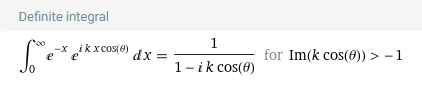
\includegraphics[scale=.5]{rw-p4-int1.png}
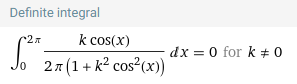
\includegraphics[scale=.5]{rw-p4-int2.png}

This means 
$$\lambda(\textbf{k})=\frac{1}{2\pi}\int_{0}^{2\pi} \frac{1}{1+k^2\cos(\theta)^2}\,d\theta=\frac{1}{\sqrt{k^2+1}}$$
Now we can compute the quadratic taylor approximation which is $\lambda(\textbf{k})=\frac{1}{\sqrt{k^2+1}}\approx 1-\frac{k^2}{2}\approx\exp(-\frac{1}{2}k^2)=\exp(-\frac{1}{2}\textbf{k}^\intercal\Sigma\textbf{k})$. where $\Sigma=\begin{pmatrix} 1 & 0\\ 0 & 1 \end{pmatrix}$
Which again means that $\lambda(\textbf{k})^n=\exp(-\frac{1}{2}\textbf{k}^\intercal\Sigma\textbf{k})^n=\exp(-\frac{1}{2}\textbf{k}^\intercal n\Sigma\textbf{k})$, where $n\Sigma=\begin{pmatrix} n & 0\\ 0 & n \end{pmatrix}$.\\

This is a common characteristic function(Source: \href{https://en.wikipedia.org/wiki/Multivariate_normal_distribution}{here}) so we know that
$P_n(x)$ is the probability density function of $\mathcal{N}(0, n\Sigma)$, which is $P_n(\textbf{x})=\det(2\pi n\Sigma)^{-\frac{1}{2}}\exp(-\frac{1}{2}\textbf{x}^\intercal n\Sigma \textbf{x})=\frac{1}{\sqrt{2\pi}n}\exp(-\frac{1}{2}\textbf{x}^\intercal n\Sigma \textbf{x})$.\\

\item[(5)] 
First for problem 2 in which we are looking at a random walk on a square lattice. I generated a random walk with $300$ steps, with the start labeled in blue and the end labeled in orange.\\
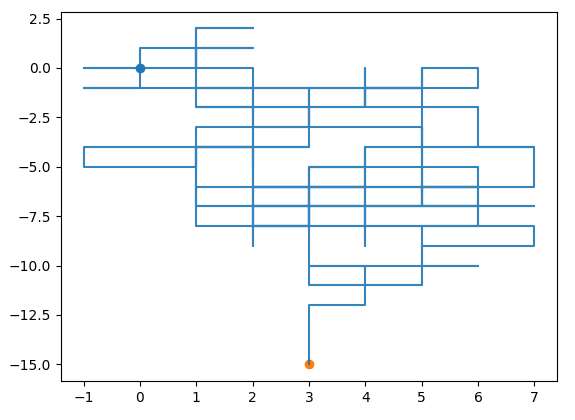
\includegraphics[scale=.5]{rw-p5p2.png}

Now for problem 3 in which we are looking at a radially symmetric random walk on continuous space with jumps of length $l=1$. I generated a random walk with $300$ steps, with the start labeled in blue and the end labeled in orange.\\
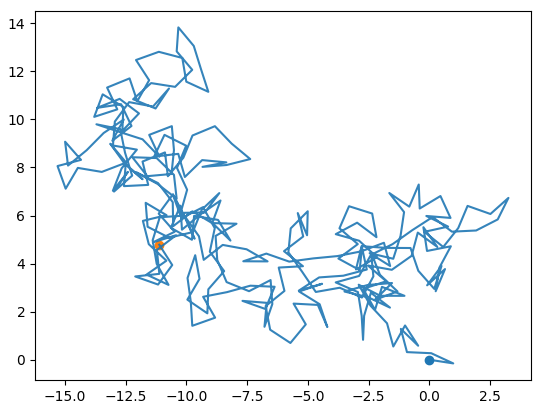
\includegraphics[scale=.5]{rw-p5p3.png}

Finally for problem 4 in which we are looking at a radially symmetric random walk on continuous space with jumps from an exponential distribution. I generated a random walk with $300$ steps, with the start labeled in blue and the end labeled in orange.\\
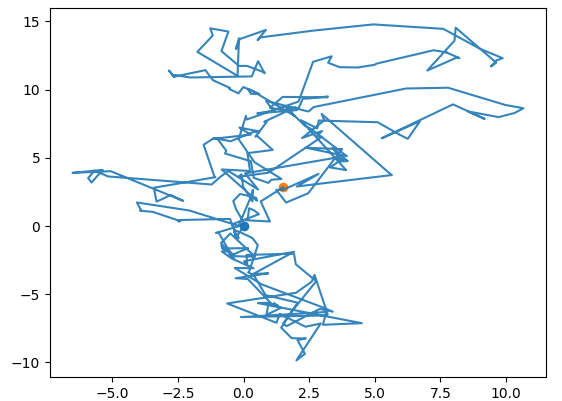
\includegraphics[scale=.5]{rw-p5p4.png}

The code used to generate each random walk is provided below. Additionally the trajectories for each random walk have been added as separate files labeled: ian-rw-p5-2.txt, ian-rw-p5-3.txt, and ian-rw-p5-4.txt

\newpage
\section*{Appendix}
\lstinputlisting[language=Python]{randomwalks.py}








\end{itemize}

\end{document}


